\chapter{About nJexl}\label{nJexl}

{\LARGE A} philosophy is needed to guide the design of any system. nJexl is not much different.
Here we discuss the rationale behind the language, and showcase how it is distinct from its first cousin Java.
While it is reasonably close to Scala is not a surprise, that is an example of convergent evolution.

\begin{section}{nJexl Philosophy}
\index{philosophy}

My experience in Industry is aptly summarized by \href{https://en.wikipedia.org/wiki/Node.js}{Ryan Dahl}
in \href{http://harmful.cat-v.org/software/node.js}{here} , the creator of Node.js :

\begin{center}
\emph{
I hate almost all software. It's unnecessary and complicated at almost every layer. At best I can congratulate someone for quickly and simply solving a problem on top of the shit that they are given. The only software that I like is one that I can easily understand and solves my problems. The amount of complexity I'm willing to tolerate is proportional to the size of the problem being solved...(continued)...
Those of you who still find it enjoyable to learn the details of, say, a programming language - being able to happily recite off if NaN equals or does not equal null - you just don't yet understand how utterly fucked the whole thing is. If you think it would be cute to align all of the equals signs in your code, if you spend time configuring your window manager or editor, if put unicode check marks in your test runner, if you add unnecessary hierarchies in your code directories, if you are doing anything beyond just solving the problem - you don't understand how fucked the whole thing is. No one gives a fuck about the glib object model.
\emph{The only thing that matters in software is the experience of the user.}   - Ryan Dahl
}
\end{center}

Thus, nJexl comes with it's tenets, which are :

\begin{enumerate}
\item{ Reduce the number of lines in the code; }
\item{ If possible, in every line, reduce the number of characters; }
\item{ To boldly go where no developer has gone before - attaining Nirvana in terms of coding;
    - get out of the cycle of bugs and fixes by writing scientific code 
    ( see  \href{http://en.wikipedia.org/wiki/Minimum_description_length}{Minimum Description length} ).
\item{Good code is, once written, forever forgotten, i.e. : limiting to 0 maintenance. }    
}
\end{enumerate}

Thus I made nJexl so that a language exists with it's full focus on \emph{Business Process Automation and Software Testing \& Validation},
not on commercial fads that sucks the profit out of business. Hence it has one singular focus in mind : \emph{brevity} but not on the cost of maintainability. What can be done with 1 people, in 10 days, get it done in 1 day by one person.

\end{section}

\begin{section}{Design Features}
\index{design}
Here is the important list of features, which make nJexl a first choice of the business developers and software testers, alike.

\begin{subsection}{nJexl is Embeddable}

nJexl scripts are easy to be invoked as stand alone scripts, also from within java code, 
thus making integration of external logic into proper code base easy. Thus Java code
can call nJexl scripts very easily, and all of nJexl functionality is programmatically 
accessible by Java caller code. This makes it distinct from Scala, where it is almost impossible
to call scala code from Java. Lots of code of how to call nJexl can be found 
in the \href{https://github.com/nmondal/njexl/tree/master/lang/src/test/java/com/noga/njexl/lang}{test} directory. 
Many scripts are there as samples in \href{https://github.com/nmondal/njexl/tree/master/lang/samples}{samples} folder.
In chapter -- we would showcase how to embed nJexl in Java code.
\end{subsection}

\begin{subsection}{Interpreted by JVM}

nJexl is interpreted by a program written in Java, and uses Java runtime. 
This means that nJexl and Java have a common runtime platform. 
You can easily move from Java to nJexl and vice versa.

\end{subsection}

\begin{subsection}{nJexl can Execute any Java Code}

nJexl enables you to use all the classes of the Java SDK's in nJexl, and also your own, custom Java classes, or your favourite Java open source projects. There are trivial ways to load a jar from path directly from nJexl script, and then loading a class as as trivial 
as importing the class.

\end{subsection}


\begin{subsection}{nJexl can be used Functionally}

nJexl is also a functional language in the sense that every function is a value and because every value is an object so ultimately every function is an object. Functions are first class citizens.

nJexl provides a lightweight syntax for defining anonymous functions, it supports higher-order functions, it allows functions to be nested, and supports \href{https://en.wikipedia.org/wiki/Currying}{currying} and Closures. 

\end{subsection}

\begin{subsection}{nJexl is Dynamically Typed}
nJexl, unlike other statically typed languages, does not expect you to provide type information. 
You don't have to specify a type in most cases, and you certainly don't have to repeat it.

\end{subsection}

\begin{subsection}{nJexl Vs Java}

Most of the type one can treat nJexl as a very tiny shorthand for incredibly fast programming using JVM.
However, nJexl has a set of features, which completely differs from Java. Some of these are:

\begin{enumerate}

\item{ All types are objects. An assignment of the form $x = 1 $ makes actually an Integer object in JVM, not a int. }

\item { Type inference :  by that one does not need to cast a variable to a type before accessing its functions. 
    This makes reflective calls intuitive, as $ a.b.f() $ can be written as $ a['b'].f() $ and thus, the value of $'b'$
    itself can come from another variable. Objects are treated like property buckets, as in Dictionaries.  
}

\item { Nested Functions : functions can be nested :
\begin{lstlisting}[style=JexlStyle][float]
def parent_function( a ) {
    def child_function (b) {
        // child can use parents args: happily.
    	a + b 
    }
    if ( a != null ) {
      return child_function 
   }
}
\end{lstlisting}
}

\item { Functions are objects, as the above example aptly shows, they can be returned, and assigned : 

\begin{lstlisting}[style=JexlStyle][float]
fp = parent_function(10) 
r = fp(32 ) // result will be 42.
\end{lstlisting}
}

\item{ Closures : the above example demonstrates the closure using partial functions, and this is something that is
syntactically new to Java land.}

\end{enumerate}

\end{subsection}

\end{section}

\begin{section}{Setting up Environment}

\begin{subsection}{Installing Java Run Time}

 You need to install Java runtime 1.8 ( 64 bit ).
 To test whether or not you have successfully installed it try this 
 in your command prompt :

\begin{lstlisting}
    $ java -version
    java version "1.8.0_60"
    Java(TM) SE Runtime Environment (build 1.8.0_60-b27)
    Java HotSpot(TM) 64-Bit Server VM (build 25.60-b23, mixed mode)
\end{lstlisting}

\end{subsection}

\begin{subsection}{Download nJexl one jar}

Download the latest one-jar.jar file from \href{https://oss.sonatype.org/content/repositories/snapshots/com/github/nmondal/njexl.lang/0.3-SNAPSHOT/}{here}.

\end{subsection}

\begin{subsection}{Add to Path}

If you are using \*nix platform, then you should create an alias :

\begin{lstlisting}
     alias njexl = "java -jar njexl.lang-0.3-<time-stamp>-onejar.jar" 
\end{lstlisting}

in your .login file.

If you are using Windows, then you should create a batch file that looks like this:

\begin{lstlisting}
     @echo off
     rem njexl.bat 
     java -jar njexl.lang-0.3-<time-stamp>-onejar.jar  %1 %2 %3 %4 %5 %6

\end{lstlisting}

and then add path to this njexl.bat file in your path variable, see 
\href{https://www.google.co.in/search?client=safari&rls=en&q=adding+path+in+windows&ie=UTF-8&oe=UTF-8&gfe_rd=cr&ei=EWpIVqjUJ-PI8AfWm4GgBQ}{here}.

\end{subsection}

\begin{subsection}{Test Setup}

Open a command prompt, and type :

\begin{lstlisting}
     $njexl 
     (njexl)
\end{lstlisting}     

It should produce the prompt of \href{https://en.wikipedia.org/wiki/Read?eval?print_loop}{REPL} of (njexl).

\end{subsection} 

\begin{subsection}{Maven Setup for Java Integration}
In the dependency section (latest release is 0.2 ) : 

\begin{lstlisting}
<dependency>
  <groupId>com.github.nmondal</groupId>
  <artifactId>njexl.lang</artifactId>
  <version>0.2</version> <!-- or 0.3-SNAPSHOT -->
</dependency>
\end{lstlisting}

That should immediately make your project a nJexl supported one. 
\end{subsection} 


\begin{subsection}{Setting up Editors}

IDEs are good - and that is why we have minimal editor support, \href{http://www.sublimetext.com}{Sublime Text} is my favourite one. 
You also have access to the syntax highlight file for jexl and a specially made theme for jexl editing - ( ES ) both of them can be found :   \href{https://github.com/nmondal/njexl/tree/master/doc}{here}. 
There is also a vim syntax file.
If you use them with your sublime text editor - then typical jexl script file looks like this : 

\begin{figure}
\begin{center}
\leavevmode
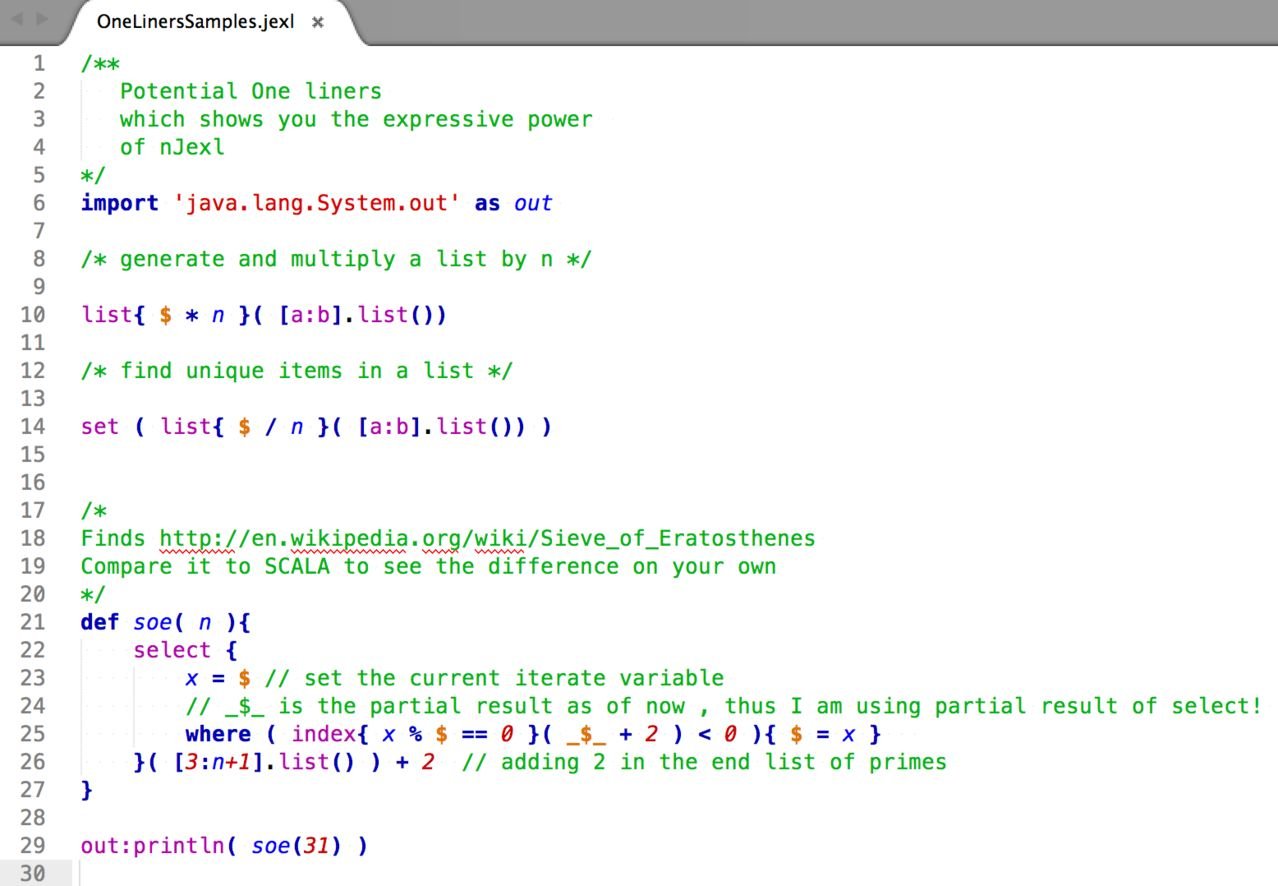
\includegraphics[scale=0.6]{sublime.jpeg}
\end{center}
\caption{Using Sublime Text}
\label{fig_2_1}
\end{figure}

To include for vim :

Create these two files :

\begin{lstlisting}
    $HOME/.vim/ftdetect/jxl.vim
    $HOME/.vim/syntax/jxl.vim
\end{lstlisting}

For most \*nix systems it would be same as :

\begin{lstlisting}
    mkdir -p ~/.vim/ftdetect/
    touch ~/.vim/ftdetect/jxl.vim 
    touch ~/.vim/syntax/jxl.vim 
\end{lstlisting}

Now on the \$HOME/.vim/ftdetect/jxl.vim  file, put this line :

\begin{lstlisting}
    autocmd BufRead,BufNewFile *.jxl,*.jexl,*.njxl,*.njexl  set filetype=jxl
\end{lstlisting}

Note that you should not have blanks between commas.
And then, copy the content of the \href{https://github.com/nmondal/njexl/blob/master/doc/jxl.vim}{vim syntax file here} 
in the \$HOME/.vim/syntax/jxl.vim file as is.

If everything is fine, you can now open jexl scripts in vim!

\end{subsection} 

\end{section}




